% =====================================================================
%  TalkToMyTwin -- Project Review Report
%  Compile on Overleaf with pdfLaTeX. Compiles with or without images:
%  any image not yet uploaded to a "figures" folder shows as a labelled box.
% =====================================================================
\documentclass[11pt,a4paper]{article}

\usepackage[T1]{fontenc}
\usepackage[utf8]{inputenc}
\usepackage{lmodern}
\usepackage[margin=2.2cm]{geometry}
\usepackage{amsmath,amssymb}
\usepackage{graphicx}
\usepackage{float}
\usepackage{booktabs}
\usepackage{tabularx}
\usepackage{longtable}
\usepackage{array}
\usepackage{multirow}
\usepackage[table]{xcolor}
\usepackage{caption}
\usepackage{subcaption}
\usepackage{enumitem}
\usepackage{listings}
\usepackage{tikz}
\usetikzlibrary{positioning,arrows.meta,fit,backgrounds,calc,shapes.geometric}
\usepackage{microtype}
\usepackage{hyperref}
\hypersetup{colorlinks=true,linkcolor=blue!50!black,citecolor=green!40!black,urlcolor=blue!60!black}

% ---- layout tweaks ----
\captionsetup{font=small,labelfont=bf,skip=4pt}
\captionsetup[sub]{font=footnotesize}
\setlength{\parskip}{3pt}
\raggedbottom

\DeclareRobustCommand{\file}[1]{\texttt{\detokenize{#1}}}
\newcolumntype{Y}{>{\raggedright\arraybackslash}X}

% ---- block-diagram styles ----
\tikzset{
  blk/.style={draw, rounded corners=2pt, align=center, minimum height=0.95cm, text width=2.7cm, fill=white},
  io/.style={blk, fill=gray!12},
  plan/.style={blk, dashed, fill=white, text=gray!70!black},
  arr/.style={-{Stealth[length=2.2mm]}, thick},
  darr/.style={-{Stealth[length=2.2mm]}, thick, dashed, gray},
  stage/.style={draw=#1!70, fill=#1!6, rounded corners=6pt, inner sep=8pt},
  lab/.style={font=\sffamily\bfseries\small, anchor=south west}
}

% ---- photo macro: finds the image either in a "figures" folder or in the
%      main project folder; if neither exists it draws a labelled box ----
% usage: \photo{width}{placeholder height}{figures/file}
\def\photobase figures/#1\relax{#1}
\newcommand{\photo}[3]{%
  \edef\photoalt{\photobase#3\relax}%
  \IfFileExists{#3}%
    {\includegraphics[width=#1]{#3}}%
    {\IfFileExists{\photoalt}%
      {\includegraphics[width=#1]{\photoalt}}%
      {\fbox{\parbox[c][#2][c]{\dimexpr #1-2\fboxsep-2\fboxrule\relax}{\centering\small
        \textit{Photo placeholder -- upload this file to Overleaf:}\\[3pt]
        \texttt{\expandafter\detokenize\expandafter{\photoalt}}}}}}%
}


\definecolor{codebg}{RGB}{247,247,247}
\definecolor{done}{RGB}{39,174,96}
\definecolor{partial}{RGB}{230,126,34}
\definecolor{todo}{RGB}{192,57,43}
\newcommand{\stDone}{\textcolor{done}{\textbf{Done}}}
\newcommand{\stPart}{\textcolor{partial}{\textbf{Partial}}}
\newcommand{\stTodo}{\textcolor{todo}{\textbf{Planned}}}

\lstdefinestyle{out}{
  basicstyle=\ttfamily\scriptsize,
  backgroundcolor=\color{codebg},
  frame=single, rulecolor=\color{gray!40},
  breaklines=true, columns=fullflexible, keepspaces=true,
  showstringspaces=false, aboveskip=6pt, belowskip=6pt
}
\lstdefinestyle{py}{
  language=Python,
  basicstyle=\ttfamily\scriptsize,
  backgroundcolor=\color{codebg},
  keywordstyle=\color{blue!60!black}\bfseries,
  commentstyle=\color{gray},
  stringstyle=\color{green!40!black},
  frame=single, rulecolor=\color{gray!40},
  breaklines=true, columns=fullflexible, keepspaces=true,
  showstringspaces=false, numbers=left, numberstyle=\tiny\color{gray}
}

% ---------------------------------------------------------------------
\title{\textbf{TalkToMyTwin}\\[4pt]
\large A Monocular-Camera Traffic Digital Twin for Vehicle Tracking,\\
Trajectory Analytics and Collision-Risk Assessment\\[10pt]
\normalsize Project Review Report}
\author{Aarav Gupta\\
\small Register No.: \underline{\hspace{3cm}} \quad Guide: \underline{\hspace{4cm}}\\
\small Department / Institute: \underline{\hspace{7cm}}}
\date{September 2026}

\begin{document}
\maketitle

\begin{abstract}
\noindent
Roadside CCTV cameras are everywhere, but their footage is mostly watched by people or not at all. This project,
\emph{TalkToMyTwin}, turns one ordinary monocular traffic video into a \emph{traffic digital twin}: a live,
metric, bird's-eye representation of the road in which every vehicle is a tracked entity with an identity,
a class, a ground-plane position and (after filtering) a velocity and an acceleration. The pipeline combines
YOLO11 object detection, BoT-SORT/TrackTrack multi-object tracking, a \emph{fully automatic} homography
calibration driven by SegFormer road segmentation, a shadow-based ground-contact refinement, and a set of
stability and anomaly gates. Every detection is written to a per-frame log, which feeds an offline analytics
layer: a constant-acceleration Kalman filter for kinematics, traffic-science EDA (lane structure, speed
distributions, headways, Edie's fundamental-diagram measures), a surrogate-safety engine (TTC, MTTC, DRAC) and
an evaluation module that exports MOTChallenge-format predictions for HOTA scoring. On a 378-frame (12.6\,s)
segment of real mixed urban traffic the twin keeps 96.4\% of all detections, runs without dropped frames on a
laptop GPU (RTX~2050), and produces synchronised 2D and 3D twin videos. The report also states the current
limitations honestly: the depth axis of the automatic calibration is compressed, so absolute speeds and
safety measures are not yet trustworthy, and ground-truth annotation for HOTA is still outstanding.
\end{abstract}

\tableofcontents
\newpage

% =====================================================================
\section{Introduction}
% =====================================================================
\subsection{Motivation}
Traffic monitoring centres depend on operators watching many camera feeds at once. Incidents such as near-misses,
stalled vehicles and build-up of congestion are easy to miss, and the video itself holds no queryable data.
A \emph{digital twin}, a virtual replica that is kept in sync with its physical counterpart~\cite{grieves2017,tao2019},
offers a different model: convert pixels into a structured, metric state of the road that software can reason about.

\subsection{Problem statement}
Given a single, uncalibrated, fixed roadside camera, build a system that
\begin{enumerate}[nosep]
  \item detects and persistently tracks every vehicle,
  \item maps each vehicle onto a metric ground plane \emph{without manual calibration},
  \item maintains a live 2D/3D twin of the road, and
  \item logs the twin state so that traffic analytics and collision-risk measures can be computed and evaluated.
\end{enumerate}

\subsection{Objectives}
\begin{itemize}[nosep]
  \item \textbf{O1} Real-time perception: detection + tracking on a consumer GPU.
  \item \textbf{O2} Automatic camera-to-ground calibration (no hand-clicked points).
  \item \textbf{O3} Robust ground-plane localisation with noise and anomaly suppression.
  \item \textbf{O4} A reproducible trajectory log and a live 2D + 3D twin visualisation.
  \item \textbf{O5} Offline analytics: kinematics, lane/speed/headway/flow statistics.
  \item \textbf{O6} Surrogate safety measures (TTC, MTTC, DRAC) for collision-risk detection.
  \item \textbf{O7} A layered evaluation protocol (perception, geometric fidelity, behavioural fidelity).
\end{itemize}

% =====================================================================
\section{Detailed Literature Review / Existing Work Survey}
% =====================================================================

\subsection{Digital twins in transportation}
The digital-twin concept originates in product lifecycle management~\cite{grieves2017}; Tao \emph{et al.}~\cite{tao2019}
survey its spread across industry and identify the three defining elements: a physical entity, a virtual model and
the data connection between them. In transportation, Ku\v{s}i\'{c} \emph{et al.}~\cite{kusic2023} build a motorway twin
that fuses live loop-detector data with a SUMO simulation~\cite{sumo2018}. Such twins are typically driven by
infrastructure sensors (loops, radar) that are expensive and sparse. Commercial smart-city stacks (e.g.\ NVIDIA
Metropolis/Omniverse) use cameras, but their pipelines are closed. \textbf{Gap:} few open works build a twin from a
\emph{single uncalibrated CCTV camera} and expose its full data path for evaluation.

\subsection{Object detection}
One-stage detectors starting with YOLO~\cite{redmon2016} made real-time detection practical. The Ultralytics YOLO11
family~\cite{yolo11} is the current widely deployed version, trained on COCO~\cite{coco2014}, whose classes include
\emph{car, motorcycle, bus, truck}. \textbf{Gap:} COCO has no class for the three-wheelers (auto-rickshaws, e-rickshaws)
that dominate South-Asian traffic, including the footage used here; they are detected as car/truck with lower confidence.

\subsection{Multi-object tracking (MOT)}
SORT~\cite{bewley2016} introduced tracking-by-detection with a Kalman filter and Hungarian assignment on IoU.
DeepSORT~\cite{wojke2017} added appearance (Re-ID) embeddings to survive occlusion. ByteTrack~\cite{zhang2022} showed
that also associating \emph{low-confidence} detections recovers occluded objects. BoT-SORT~\cite{aharon2022} adds camera
motion compensation (GMC) and Re-ID fusion. TrackTrack~\cite{shim2025} (CVPR 2025) moves to a track-focused
association with track-aware initialisation. This project uses BoT-SORT and TrackTrack configurations with Re-ID and
sparse optical-flow GMC, and a deliberately low detection threshold (0.1) so that ByteTrack-style low-score
association can operate.

\subsection{Camera calibration and inverse perspective mapping}
A planar homography maps the road plane in the image to a top-down plane~\cite{hartley2004}; applied to the whole image
it is known as Inverse Perspective Mapping (IPM)~\cite{mallot1991}. Classical calibration requires hand-picked point
correspondences with known world coordinates. Dubsk\'{a} \emph{et al.}~\cite{dubska2014} calibrate traffic cameras
automatically from vanishing points of vehicle motion, and Sochor \emph{et al.}~\cite{sochor2019} (BrnoCompSpeed) show
that automatic monocular calibration is the dominant error source in camera-based speed measurement.
Semantic segmentation with SegFormer~\cite{xie2021} trained on Cityscapes~\cite{cordts2016} gives a reliable
\emph{road} mask. \textbf{Gap:} using a learned road mask directly to \emph{place} the homography points has
received little attention; this is the approach taken here.

\subsection{Trajectory reconstruction and kinematics}
Raw camera trajectories are noisy; differentiating them amplifies noise. NGSIM-based studies~\cite{montanino2015,punzo2011}
show that unfiltered trajectory data produce physically impossible accelerations. Standard remedies are
Savitzky--Golay smoothing~\cite{savitzky1964} and Kalman filtering~\cite{kalman1960}. The highD dataset~\cite{krajewski2018}
demonstrates the quality achievable from a top-down drone view, which is the reference a roadside twin tries to approximate.

\subsection{Surrogate safety measures (SSM)}
Crashes are rare, so safety is assessed through \emph{conflicts}. Time-to-Collision (TTC) was introduced by
Hayward~\cite{hayward1972}; Post-Encroachment Time (PET) by Allen \emph{et al.}~\cite{allen1978}; Deceleration Rate
to Avoid a Crash (DRAC) follows Cooper and Ferguson~\cite{cooper1976}. Ozbay \emph{et al.}~\cite{ozbay2008} proposed
Modified TTC (MTTC), which includes relative acceleration and so remains valid while vehicles brake.
\textbf{Gap:} most SSM studies use drone or simulated trajectories; applying them to monocular CCTV twins requires
explicit handling of depth-dependent position error, which is addressed here by near/far-field tagging and
plausibility filters.

\subsection{Traffic-flow analytics and control}
Edie's generalised definitions~\cite{edie1963} give flow, density and space-mean speed over a time-space region
directly from trajectories, enabling fundamental diagrams from camera data. For signal control, Max-Pressure~\cite{varaiya2013}
is decentralised and throughput-optimal and needs only per-lane counts, which is exactly what a twin provides.
This is planned future work.

\subsection{Evaluation of MOT and twins}
CLEAR-MOT~\cite{bernardin2008} (MOTA/MOTP) and IDF1~\cite{ristani2016} were the standard until HOTA~\cite{luiten2021},
which separates detection accuracy (DetA) from association accuracy (AssA). The MOTChallenge text format~\cite{milan2016}
is the common interchange format for these tools.

\subsection{Summary of surveyed work}
\begin{table}[H]
\centering\small
\caption{Comparison of representative existing work with the proposed system.}
\label{tab:lit}
\begin{tabularx}{\textwidth}{@{}l Y Y Y@{}}
\toprule
\textbf{Work} & \textbf{Contribution} & \textbf{Limitation w.r.t.\ this problem} & \textbf{How this project uses / extends it}\\
\midrule
YOLO / YOLO11~\cite{redmon2016,yolo11} & Real-time detection & No 3-wheeler class; image-space only & Detector; outputs lifted to ground plane\\
SORT, DeepSORT~\cite{bewley2016,wojke2017} & Kalman + assignment, Re-ID & ID switches under occlusion & Baseline concept\\
ByteTrack, BoT-SORT~\cite{zhang2022,aharon2022} & Low-score association, GMC & Image-space tracks, no metric state & Tracker used in pipeline\\
TrackTrack~\cite{shim2025} & Track-focused association & New, few deployed uses & Alternative tracker config\\
IPM / homography~\cite{mallot1991,hartley2004} & Image to ground plane & Needs manual points & Automated via road mask\\
Dubsk\'{a}~\cite{dubska2014}, Sochor~\cite{sochor2019} & Automatic calibration, speed & Needs long vehicle motion & Motivates depth-scale fix (future)\\
SegFormer~\cite{xie2021} & Road segmentation & Not a calibration method & Drives automatic calibration\\
Hayward, Ozbay, Cooper~\cite{hayward1972,ozbay2008,cooper1976} & TTC, MTTC, DRAC & Assume clean trajectories & Applied with KF + noise gates\\
Edie~\cite{edie1963} & Flow/density from trajectories & Needs metric trajectories & Implemented on twin log\\
Ku\v{s}i\'{c}~\cite{kusic2023} & Motorway twin + SUMO & Loop detectors, not cameras & Camera-only twin\\
HOTA~\cite{luiten2021} & Balanced MOT metric & Needs ground truth & MOT export ready\\
\bottomrule
\end{tabularx}
\end{table}

\subsection{Literature survey of 22 works}
Table~\ref{tab:survey22} surveys 22 papers in the order of the pipeline: digital twins, detection, tracking,
datasets, road segmentation and calibration, trajectory quality, safety measures, evaluation and traffic control.
For each paper it lists the method, the main finding, and the gap that this project addresses or the way it uses the work.

{\footnotesize
\setlength{\tabcolsep}{3pt}
\renewcommand{\arraystretch}{1.15}
\begin{longtable}{@{}>{\raggedright\arraybackslash}p{0.4cm}>{\raggedright\arraybackslash}p{2.7cm}>{\raggedright\arraybackslash}p{4.3cm}>{\raggedright\arraybackslash}p{3.9cm}>{\raggedright\arraybackslash}p{4.3cm}@{}}
\caption{Literature survey of 22 works.}\label{tab:survey22}\\
\toprule
\textbf{\#} & \textbf{Authors (Year)} & \textbf{Method / contribution} & \textbf{Key finding} & \textbf{Gap / relevance to this project}\\
\midrule\endfirsthead
\toprule
\textbf{\#} & \textbf{Authors (Year)} & \textbf{Method / contribution} & \textbf{Key finding} & \textbf{Gap / relevance to this project}\\
\midrule\endhead
\midrule\multicolumn{5}{r}{\textit{continued on next page}}\\\endfoot
\bottomrule\endlastfoot
\multicolumn{5}{@{}l}{\textit{A. Digital twins}}\\
1 & Grieves \& Vickers (2017)~\cite{grieves2017} & Defines the digital twin as physical product, virtual product and the data link between them. & Twins can expose unpredictable emergent behaviour before it occurs in the real system. & Conceptual only. This project realises the ``data link'' as a per-frame trajectory log.\\
2 & Tao \emph{et al.} (2019)~\cite{tao2019} & State-of-the-art survey of digital twins in industry. & Identifies modelling, data fusion and real-time synchronisation as the core challenges. & Transportation is under-represented. Motivates a real-time, data-synchronised traffic twin.\\
3 & Ku\v{s}i\'{c} \emph{et al.} (2023)~\cite{kusic2023} & Motorway digital twin that feeds live traffic-detector streams into a SUMO simulation. & Real-time synchronisation of the simulation with measured traffic is feasible. & Uses fixed infrastructure sensors. This project builds the twin from one uncalibrated camera instead.\\
\multicolumn{5}{@{}l}{\textit{B. Detection and tracking}}\\
4 & Redmon \emph{et al.} (2016)~\cite{redmon2016} & YOLO: detection as a single regression over a grid, in one network pass. & Real-time detection with competitive accuracy. & Image-space boxes only. Here the boxes are lifted to a metric ground plane (YOLO11s).\\
5 & Bewley \emph{et al.} (2016)~\cite{bewley2016} & SORT: Kalman-filter motion model plus Hungarian assignment on IoU. & Simple tracking-by-detection runs at very high frame rates. & Many ID switches under occlusion. Basis of the trackers used here.\\
6 & Wojke \emph{et al.} (2017)~\cite{wojke2017} & DeepSORT: adds a deep appearance (Re-ID) descriptor to SORT. & Fewer ID switches through long occlusions. & Re-ID is enabled in this project's tracker configs.\\
7 & Zhang \emph{et al.} (2022)~\cite{zhang2022} & ByteTrack: also associates low-confidence detections in a second matching stage. & Recovers occluded objects; top results on MOT17/MOT20. & Motivates this project's low detection floor (conf $=0.1$).\\
8 & Aharon \emph{et al.} (2022)~\cite{aharon2022} & BoT-SORT: camera-motion compensation, improved Kalman state, IoU--Re-ID fusion. & State-of-the-art MOT17/MOT20 results at the time of publication. & Main tracker in \file{digital_twin_log.py}.\\
9 & Shim \emph{et al.} (2025)~\cite{shim2025} & TrackTrack: track-focused association and track-aware initialisation. & Better online MOT through reasoning at the track level. & Alternative tracker in \file{digital_twin_live.py}.\\
\multicolumn{5}{@{}l}{\textit{C. Datasets for traffic scenes}}\\
10 & Tang \emph{et al.} (2019)~\cite{tang2019} & CityFlow: city-scale multi-camera vehicle tracking and re-identification benchmark. & Real intersection CCTV footage is much harder than standard MOT benchmarks. & Western traffic only. Future multi-camera extension of this twin.\\
11 & Varma \emph{et al.} (2019)~\cite{varma2019} & IDD: Indian driving dataset with a label set that includes auto-rickshaws. & Unstructured Indian roads differ strongly from Cityscapes-style scenes. & Candidate data for fine-tuning on three-wheelers, a COCO gap seen in this project.\\
12 & Krajewski \emph{et al.} (2018)~\cite{krajewski2018} & highD: drone-recorded naturalistic trajectories on German highways. & Top-down video yields high-quality trajectories of about 110{,}000 vehicles. & Shows the quality a roadside twin should approach. Here a tilted CCTV view is used instead of a drone.\\
\multicolumn{5}{@{}l}{\textit{D. Road segmentation and calibration}}\\
13 & Xie \emph{et al.} (2021)~\cite{xie2021} & SegFormer: hierarchical transformer encoder with a lightweight MLP decoder. & Strong mIoU on Cityscapes at a good efficiency trade-off. & Used here (B2) to obtain the road mask that drives automatic calibration.\\
14 & Mallot \emph{et al.} (1991)~\cite{mallot1991} & Inverse perspective mapping onto the ground plane. & IPM simplifies optical-flow and obstacle computation. & Requires known camera geometry. Here the mapping is found automatically.\\
15 & Dubsk\'{a} \emph{et al.} (2015)~\cite{dubska2014} & Fully automatic roadside camera calibration from vanishing points of vehicle motion. & Automatic calibration is accurate enough for traffic measurement. & Planned fix for this project's compressed depth scale.\\
16 & Sochor \emph{et al.} (2019)~\cite{sochor2019} & BrnoCompSpeed: videos with reference speeds for monocular speed measurement. & Calibration, especially scale, is the dominant source of speed error. & Explains this project's under-estimated speeds. Suggested validation protocol.\\
\multicolumn{5}{@{}l}{\textit{E. Trajectory quality}}\\
17 & Montanino \& Punzo (2015)~\cite{montanino2015} & Multi-step reconstruction of noisy NGSIM trajectories, validated through simulation. & Raw trajectories give physically impossible speeds and accelerations until filtered. & Motivates Kalman filtering and plausibility floors before computing kinematics.\\
\multicolumn{5}{@{}l}{\textit{F. Surrogate safety measures}}\\
18 & Hayward (1972)~\cite{hayward1972} & Time-to-collision as a scale of danger for near-misses. & TTC separates dangerous from safe interactions. & Assumes constant speed and a single path. Here a 2D closest-approach TTC is used.\\
19 & Ozbay \emph{et al.} (2008)~\cite{ozbay2008} & Modified TTC (MTTC) that includes relative acceleration. & MTTC captures conflicts that TTC misses when vehicles brake or accelerate. & Implemented in \file{ttc.py} using Kalman-filtered acceleration.\\
\multicolumn{5}{@{}l}{\textit{G. Evaluation}}\\
20 & Luiten \emph{et al.} (2021)~\cite{luiten2021} & HOTA: a single metric decomposed into detection (DetA) and association (AssA). & Balances detection and association better than MOTA or IDF1 alone. & Headline metric; MOT export already produced, ground truth pending.\\
\multicolumn{5}{@{}l}{\textit{H. Traffic control}}\\
21 & Varaiya (2013)~\cite{varaiya2013} & Max-Pressure signal control from queue differences between incoming and outgoing links. & Decentralised and provably throughput-optimal. & Needs per-lane counts, which the twin produces. Planned control baseline.\\
22 & Wei \emph{et al.} (2018)~\cite{wei2018} & IntelliLight: deep reinforcement learning for traffic-light control, tested on real data. & Learned policies can outperform fixed-time control. & Needs a simulator and accurate state. The twin can supply that state; Max-Pressure is the baseline to beat.\\
\end{longtable}}

% =====================================================================
\section{Overview of the Proposed Work}
% =====================================================================
The system has three stages that run at different times and communicate through files
(Figure~\ref{fig:block}):

\begin{enumerate}[nosep]
  \item \textbf{Offline calibration} (once per camera): select the frame with the most visible road, segment the road,
        fit the road edges and compute the homography $H$ (\file{homography.npy}).
  \item \textbf{Online perception and twin} (every frame): detect, track, localise on the ground plane, filter,
        render the 2D and 3D twin, and log every detection to \file{tracking_log.csv}.
  \item \textbf{Offline analytics and evaluation} (on the log): Kalman kinematics, EDA, surrogate safety measures,
        coverage/quality evaluation and MOT export.
\end{enumerate}
Dashed blocks are the planned later phases (alert engine, database, conversational interface, signal control).

\begin{figure}[H]
\centering
\resizebox{\textwidth}{!}{%
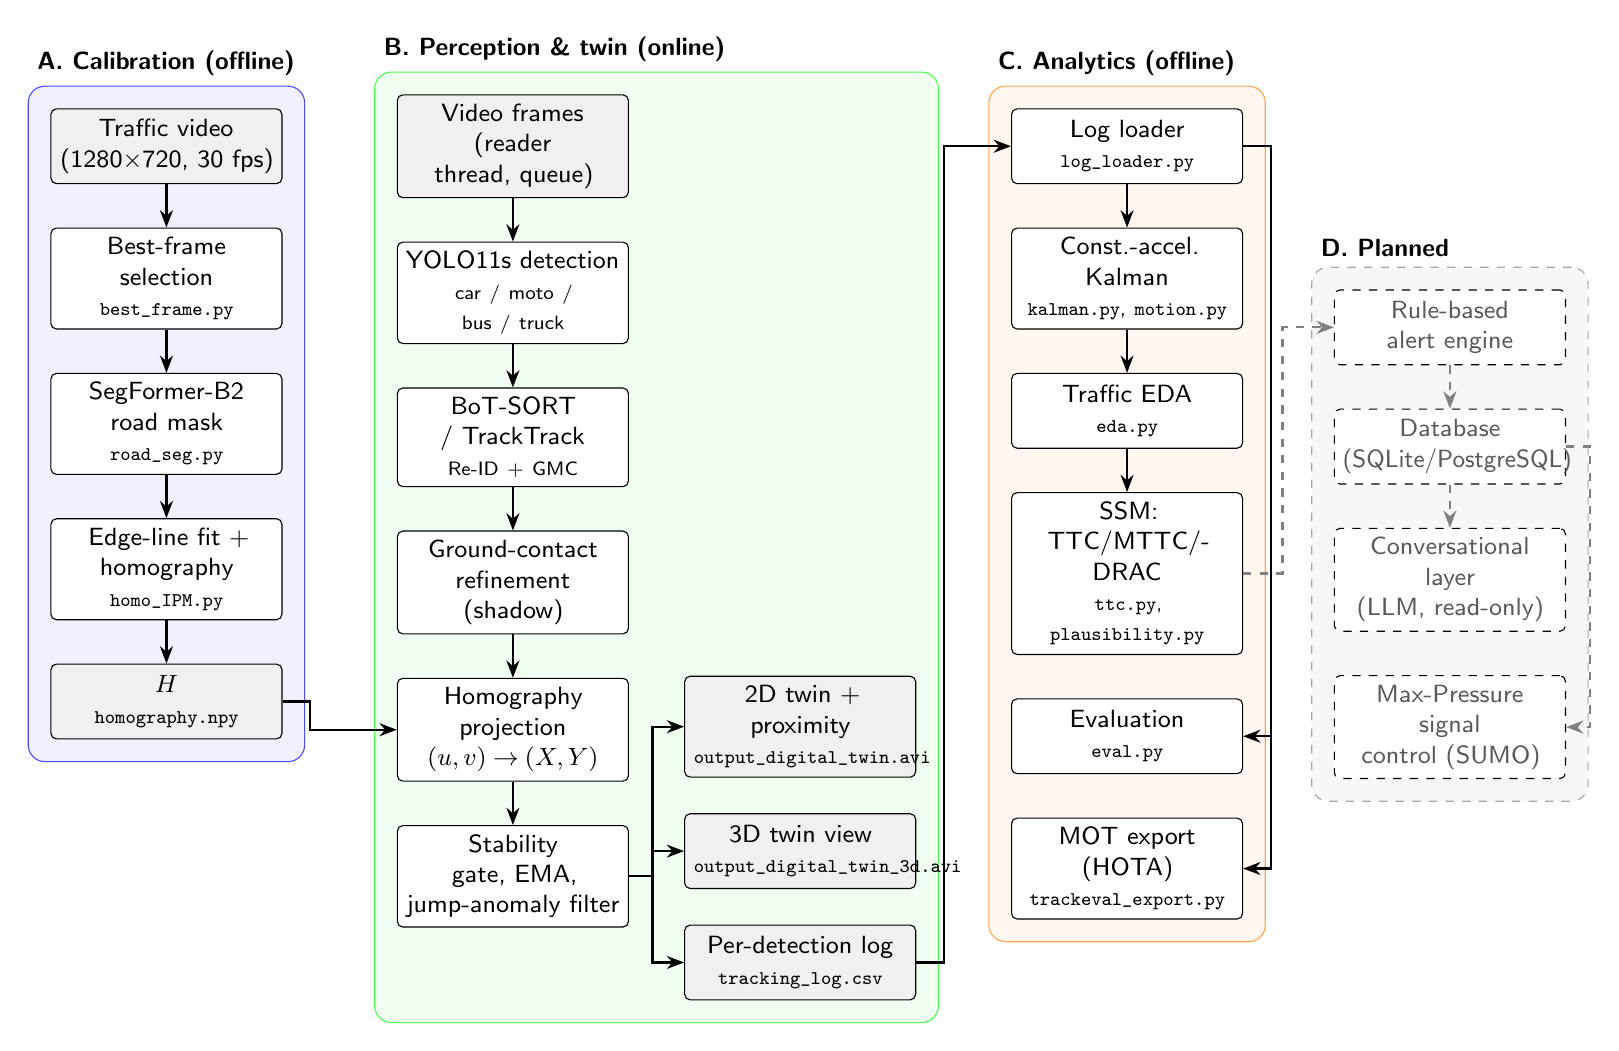
\begin{tikzpicture}[font=\sffamily\small]
% --- Stage A: calibration
\node[io]  (vid0) at (0,0) {Traffic video\\(1280$\times$720, 30 fps)};
\node[blk, below=0.55cm of vid0] (best) {Best-frame selection\\\scriptsize\file{best_frame.py}};
\node[blk, below=0.55cm of best] (seg)  {SegFormer-B2 road mask\\\scriptsize\file{road_seg.py}};
\node[blk, below=0.55cm of seg]  (ipm)  {Edge-line fit + homography\\\scriptsize\file{homo_IPM.py}};
\node[io,  below=0.55cm of ipm]  (H)    {$H$ \\\scriptsize\file{homography.npy}};
\draw[arr] (vid0)--(best); \draw[arr] (best)--(seg); \draw[arr] (seg)--(ipm); \draw[arr] (ipm)--(H);

% --- Stage B: online
\node[io]  (vid1) at (4.4,0) {Video frames\\(reader thread, queue)};
\node[blk, below=0.55cm of vid1] (det) {YOLO11s detection\\\scriptsize car / moto / bus / truck};
\node[blk, below=0.55cm of det]  (trk) {BoT-SORT / TrackTrack\\\scriptsize Re-ID + GMC};
\node[blk, below=0.55cm of trk]  (gp)  {Ground-contact\\refinement (shadow)};
\node[blk, below=0.55cm of gp]   (proj){Homography projection\\$(u,v)\!\to\!(X,Y)$};
\node[blk, below=0.55cm of proj] (gate){Stability gate, EMA,\\jump-anomaly filter};
\draw[arr] (vid1)--(det); \draw[arr] (det)--(trk); \draw[arr] (trk)--(gp); \draw[arr] (gp)--(proj); \draw[arr] (proj)--(gate);
\draw[arr] (H.east) -- ++(0.35,0) |- (proj.west);

\node[io, right=0.7cm of gate, yshift=1.9cm] (tw2) {2D twin + proximity\\\scriptsize\file{output_digital_twin.avi}};
\node[io, below=0.45cm of tw2] (tw3) {3D twin view\\\scriptsize\file{output_digital_twin_3d.avi}};
\node[io, below=0.45cm of tw3] (log) {Per-detection log\\\scriptsize\file{tracking_log.csv}};
\draw[arr] (gate.east) -- ++(0.3,0) |- (tw2.west);
\draw[arr] (gate.east) -- ++(0.3,0) |- (tw3.west);
\draw[arr] (gate.east) -- ++(0.3,0) |- (log.west);

% --- Stage C: analytics
\node[blk] (ld)  at (12.2,0) {Log loader\\\scriptsize\file{log_loader.py}};
\node[blk, below=0.55cm of ld]  (kf)  {Const.-accel.\ Kalman\\\scriptsize\file{kalman.py}, \file{motion.py}};
\node[blk, below=0.55cm of kf]  (eda) {Traffic EDA\\\scriptsize\file{eda.py}};
\node[blk, below=0.55cm of eda] (ttc) {SSM: TTC/MTTC/DRAC\\\scriptsize\file{ttc.py}, \file{plausibility.py}};
\node[blk, below=0.55cm of ttc] (ev)  {Evaluation\\\scriptsize\file{eval.py}};
\node[blk, below=0.55cm of ev]  (mot) {MOT export (HOTA)\\\scriptsize\file{trackeval_export.py}};
\draw[arr] (ld)--(kf); \draw[arr] (kf)--(eda); \draw[arr] (eda)--(ttc);
\draw[arr] (ld.east) -- ++(0.35,0) |- (ev.east);
\draw[arr] (ld.east) -- ++(0.35,0) |- (mot.east);
\draw[arr] (log.east) -- ++(0.35,0) |- (ld.west);

% --- Stage D: planned
\node[plan] (al) at (16.3,-2.3) {Rule-based alert engine};
\node[plan, below=0.55cm of al] (db) {Database\\(SQLite/PostgreSQL)};
\node[plan, below=0.55cm of db] (llm){Conversational layer\\(LLM, read-only)};
\node[plan, below=0.55cm of llm](sig){Max-Pressure signal\\control (SUMO)};
\draw[darr] (ttc.east) -- ++(0.5,0) |- (al.west);
\draw[darr] (al)--(db); \draw[darr] (db)--(llm); \draw[darr] (db.east) -- ++(0.3,0) |- (sig.east);

\begin{scope}[on background layer]
  \node[stage=blue, fit=(vid0)(H)] (sA) {};
  \node[stage=green, fit=(vid1)(gate)(tw2)(log)] (sB) {};
  \node[stage=orange, fit=(ld)(mot)] (sC) {};
  \node[stage=gray, fit=(al)(sig), dashed] (sD) {};
\end{scope}
\node[lab] at (sA.north west) {A. Calibration (offline)};
\node[lab] at (sB.north west) {B. Perception \& twin (online)};
\node[lab] at (sC.north west) {C. Analytics (offline)};
\node[lab] at (sD.north west) {D. Planned};
\end{tikzpicture}}
\caption{Block diagram of TalkToMyTwin. Solid blocks are implemented; dashed blocks are planned phases.}
\label{fig:block}
\end{figure}

% =====================================================================
\section{Proposed Methodology}
% =====================================================================

\subsection{Automatic homography calibration (Stage A)}
\paragraph{Best calibration frame.} (\file{best_frame.py})
Every 10th frame of the video is segmented and the frame with the largest road-pixel area is kept. This picks the
moment when the fewest vehicles occlude the road, which gives the cleanest road boundary.

\paragraph{Road segmentation.} (\file{road_seg.py})
SegFormer-B2 fine-tuned on Cityscapes~\cite{xie2021,cordts2016} predicts per-pixel classes; class~0 (\emph{road}) is kept.
The top 10\% of the image (sky) is cleared, the mask is cleaned with morphological closing (2 iterations) and opening
(1 iteration) using a $9\times9$ elliptical kernel, and the convex hull of the largest contour is returned.

\paragraph{Road-edge fitting and homography.} (\file{homo_IPM.py})
Instead of four hand-clicked points:
\begin{enumerate}[nosep]
  \item the \emph{bottom row} is the lowest row (below 60\% of image height) where the road is at least 200\,px wide;
  \item the \emph{top row} is searched within $\pm 60$\,px of 42\% image height for a row at least 80\,px wide;
  \item for every row between them the left-most and right-most road pixels are collected and a line
        $x = m\,y + c$ is fitted to each side by least squares, then \emph{refitted after rejecting residuals beyond $2\sigma$};
  \item the four intersections of the two edge lines with the two rows, inset by 8\,px, are the source points.
\end{enumerate}
The destination rectangle has width $W = 7.0\,\text{m} \times 120\,\text{px/m} = 840$ (a standard two-lane road width)
and height $W\cdot\rho$, where $\rho$ is the pixel aspect ratio of the source trapezoid. The homography is
\begin{equation}
  \begin{bmatrix} X' \\ Y' \\ w \end{bmatrix} = H \begin{bmatrix} u \\ v \\ 1 \end{bmatrix},\qquad
  (X,Y) = \left(\tfrac{X'}{w}, \tfrac{Y'}{w}\right),
\end{equation}
solved from the four correspondences with \texttt{cv2.getPerspectiveTransform}. The matrix obtained for the test camera is
\begin{equation}
H = \begin{bmatrix}
0.9596 & 0.0345 & -27.70\\
0 & 1.1183 & -337.72\\
0 & 7.287\times10^{-4} & 1
\end{bmatrix}.
\end{equation}
Figure~\ref{fig:calib} shows the automatically found polygon and the resulting bird's-eye view.

\subsection{Online perception and twin (Stage B)}
\paragraph{Concurrency.} A reader thread decodes frames into a bounded queue (size 4) while the main thread runs inference,
so disk I/O never stalls the GPU. The model is warmed up with 5 dummy inferences, and cuDNN benchmark/TF32 are enabled.

\paragraph{Detection and tracking.} YOLO11s runs at \texttt{imgsz=1280} on COCO classes $\{2,3,5,7\}$ with a confidence
floor of 0.1. The tracker is BoT-SORT (\file{digital_twin_log.py}) or TrackTrack with Re-ID
(\file{digital_twin_live.py}, \file{tracktrack_reid_loose.yaml}); both use sparse optical-flow GMC to compensate camera shake.

\paragraph{Ground-contact refinement.} The bottom-centre of a bounding box is a poor estimate of where the vehicle touches
the road, because boxes include shadows and are loose. For a box of height $h$, a band from $y_1+0.6h$ to $y_2+0.15h$
is cropped, the central 30--70\% of columns is taken, and the \emph{lowest row darker than the band mean} (the tyre/shadow
line) is used as the contact row:
\begin{equation}
  v_g = y_{\text{top}} + \max\{\,r : \bar{I}(r) < \operatorname{mean}_r \bar{I}(r)\,\}, \qquad u_g = \tfrac{x_1+x_2}{2}.
\end{equation}

\paragraph{Confidence zoning.} The calibrated region is back-projected with $H^{-1}$; detections in the top 35\% of its image
height are flagged \texttt{low\_conf} (far field), because a one-pixel error there corresponds to a large ground distance.

\paragraph{Gating and smoothing.} A detection is drawn only if (i) its track has been seen for at least 2 frames
(\emph{stable}) and (ii) it lies inside the padded canvas (\emph{in bounds}). Positions are smoothed with an exponential moving
average, $\mathbf{p}_t = \alpha\,\mathbf{z}_t + (1-\alpha)\,\mathbf{p}_{t-1}$ with $\alpha = 0.4$.

\paragraph{Jump-anomaly filter.} For each track the last 8 step lengths are stored. A step $d_t$ is anomalous (an ID swap or
projection glitch) if
\begin{equation}
  d_t > 0.125\,\text{m} \quad\text{and}\quad d_t > 6 \cdot \operatorname{median}(d_{t-8..t-1}),
\end{equation}
in which case no heading arrow is drawn and the step is not added to the history.

\paragraph{Twin outputs.} The 2D twin shows each vehicle as a dot (green = near field, orange = far field), its ID, a heading
arrow, and red proximity lines with distances for all pairs closer than 2.5\,m (vectorised $O(n^2)$ distance matrix). A live
Matplotlib 3D view renders the same state on a single road plane, coloured by class. Every detection, gated or not, is appended
to the log with 14 fields (source, frame, track, class, confidence, box, $X$, $Y$, low\_conf, in\_bounds, stable).

\subsection{Offline analytics (Stage C)}
\paragraph{Kinematics.} (\file{kalman.py}, \file{motion.py}) Each track's $X$ and $Y$ (converted to metres, time $t=\text{frame}/30$)
are filtered independently by a constant-acceleration Kalman filter with state $\mathbf{s}=[p,\,v,\,a]^\top$:
\begin{equation}
F=\begin{bmatrix}1&\Delta t&\tfrac12\Delta t^2\\0&1&\Delta t\\0&0&1\end{bmatrix},\quad
Q=q\begin{bmatrix}\tfrac{\Delta t^4}{4}&\tfrac{\Delta t^3}{2}&\tfrac{\Delta t^2}{2}\\ \tfrac{\Delta t^3}{2}&\Delta t^2&\Delta t\\ \tfrac{\Delta t^2}{2}&\Delta t&1\end{bmatrix},\quad
H_{\!m}=[1\;0\;0],
\end{equation}
with $q=1.0$, $R=0.05$. Using the true $\Delta t$ between observations handles missed frames naturally, and the filter directly
yields acceleration, which MTTC needs.

\paragraph{Traffic EDA.} (\file{eda.py})
\begin{itemize}[nosep]
  \item \emph{Lane structure}: 1\,m histogram of lateral position $X$; one mode per lane is expected.
  \item \emph{Speed distribution} per class, with a 2\,km/h plausibility floor (\file{plausibility.py}).
  \item \emph{Headway}: crossing times at a virtual detector line (median $Y$), by linear interpolation between frames.
  \item \emph{Temporal profile}: active tracks, detections and mean speed in 5\,s bins.
  \item \emph{Fundamental diagram} with Edie's definitions~\cite{edie1963} over a 10\,m $\times$ 5\,s cell $A$:
  \begin{equation}
     q = \frac{\sum_i d_i}{|A|},\qquad k = \frac{\sum_i t_i}{|A|},\qquad \bar v_s = \frac{q}{k},
  \end{equation}
  where $d_i$ and $t_i$ are the distance travelled and time spent by vehicle $i$ inside the cell.
\end{itemize}

\paragraph{Surrogate safety measures.} (\file{ttc.py})
For every pair $(a,b)$ in a frame, with relative position $\Delta\mathbf{p}$, velocity $\Delta\mathbf{v}$ and acceleration
$\Delta\mathbf{a}$ from the Kalman filter:
\begin{align}
  \text{TTC}_{\text{ca}} &= -\frac{\Delta\mathbf{p}\cdot\Delta\mathbf{v}}{\lVert\Delta\mathbf{v}\rVert^2}
      \quad(\text{time of closest approach; only if } \Delta\mathbf{p}\cdot\Delta\mathbf{v}<0),\\
  d_{\min} &= \lVert \Delta\mathbf{p} + \text{TTC}_{\text{ca}}\,\Delta\mathbf{v}\rVert,
\end{align}
and a warning is raised when $0 < \text{TTC}_{\text{ca}} \le 3$\,s and $d_{\min} \le 2.5$\,m. This 2D closest-approach
form works for any pair of headings, not only leader--follower pairs. For each warning:
\begin{itemize}[nosep]
  \item \textbf{MTTC}~\cite{ozbay2008}: with range $d_0=\lVert\Delta\mathbf{p}\rVert$, range rate $r'=\Delta\mathbf{p}\cdot\Delta\mathbf{v}/d_0$ and
        $r''=(\lVert\Delta\mathbf{v}\rVert^2+\Delta\mathbf{p}\cdot\Delta\mathbf{a}-r'^2)/d_0$, MTTC is the smallest positive root of
        $d_0 + r' t + \tfrac12 r'' t^2 = 0$.
  \item \textbf{DRAC}~\cite{cooper1976}: $\text{DRAC} = r'^2 / (2 d_0)$, compared with a maximum available deceleration
        MADR $=3.4$\,m/s$^2$.
\end{itemize}
Noise gates: pairs closer than 0.5\,m for 3 or more frames are treated as \emph{duplicate tracks of one vehicle} and excluded;
single-frame distances under 10\,cm are rejected as implausible; every event is tagged near-field or far-field.

\subsection{Evaluation protocol}
Evaluation is split into three layers:
\begin{enumerate}[nosep]
  \item \textbf{Perception}: HOTA/DetA/AssA, IDF1, ID switches~\cite{luiten2021,ristani2016}. \file{trackeval_export.py}
        writes predictions in MOTChallenge format; ground-truth annotation is the next step.
  \item \textbf{Geometric fidelity}: coverage of the calibrated region, reprojection error on unused landmarks, scale checks with
        lane-marking lengths, speed error against manually timed vehicles.
  \item \textbf{Behavioural fidelity}: counts, mean speed and class mix against manual counts.
\end{enumerate}
\file{eval.py} currently implements coverage, completeness, track-length, per-class and near/far breakdowns.

\subsection{Novelty and contributions}
\begin{enumerate}[nosep]
  \item \textbf{Calibration without manual clicks.} Homography points are derived from a SegFormer road mask with robust
        ($2\sigma$-refit) road-edge line fitting on the automatically chosen least-occluded frame.
  \item \textbf{Shadow-based ground-contact refinement} instead of the bounding-box bottom, which reduces the systematic
        forward bias of projected positions.
  \item \textbf{Layered noise control}: track-age gate, EMA smoothing, median-multiple jump-anomaly rejection, depth-based
        confidence zoning, duplicate-track suppression and physical plausibility floors, each targeting a specific
        monocular failure mode.
  \item \textbf{2D closest-approach TTC with Kalman-derived MTTC and DRAC}, usable for crossing as well as car-following
        conflicts in heterogeneous traffic.
  \item \textbf{A traceable data path}: one per-detection log links every twin frame, every analytics number and every
        safety event back to a video frame and bounding box, and exports directly to standard MOT evaluation tools.
  \item \textbf{Real mixed traffic}: tested on a South-Asian urban road dominated by three-wheelers, which is harder than the
        highway footage used in most twin papers.
\end{enumerate}

% =====================================================================
\section{Implementation and Demonstration}
% =====================================================================

\subsection{Environment}
\begin{table}[H]
\centering\small
\begin{tabular}{@{}ll@{}}
\toprule
Hardware & NVIDIA GeForce RTX 2050 (laptop GPU), CUDA \\
Language & Python 3 \\
Libraries & PyTorch, Ultralytics (YOLO11s), HuggingFace Transformers (SegFormer-B2), OpenCV, NumPy, Pandas, Matplotlib \\
Input & \file{Weast (1).mp4}: 1280$\times$720, 30 fps, 5102 frames (170 s) \\
Logged run & 378 frames (12.6 s), 2494 detections, 90 track IDs \\
\bottomrule
\end{tabular}
\end{table}

\subsection{Project files}
{\small
\begin{longtable}{@{}p{5.0cm}p{1.0cm}p{9.4cm}@{}}
\caption{Every file in the project folder and its role.}\label{tab:files}\\
\toprule
\textbf{File} & \textbf{Lines} & \textbf{Purpose}\\
\midrule\endfirsthead
\toprule
\textbf{File} & \textbf{Lines} & \textbf{Purpose}\\
\midrule\endhead
\file{road_seg.py} & 100 & SegFormer-B2 road mask, morphology, convex hull.\\
\file{best_frame.py} & 55 & Picks the frame with maximum road area; writes \file{calibration_frame.jpg}.\\
\file{homo_IPM.py} & 151 & Automatic 4-point selection via edge-line fitting; computes and saves $H$.\\
\file{homography.npy} & -- & Saved $3\times3$ homography matrix.\\
\file{digital_twin_live.py} & 312 & Live pipeline with TrackTrack Re-ID; 2D twin + recording.\\
\file{digital_twin_log.py} & 426 & Main pipeline: BoT-SORT, 2D twin, live 3D twin, CSV logging, three output videos.\\
\file{botsort_reid.yaml} & 14 & BoT-SORT config with Re-ID and sparse optical-flow GMC.\\
\file{tracktrack_reid.yaml} & 24 & TrackTrack config (strict thresholds).\\
\file{tracktrack_reid_loose.yaml} & 24 & TrackTrack config (low thresholds for small/far vehicles).\\
\file{log_loader.py} & 22 & Typed CSV loader shared by all analytics scripts.\\
\file{kalman.py} & 38 & 1-D constant-acceleration Kalman filter.\\
\file{motion.py} & 37 & Per-track kinematics $(x,y,v_x,v_y,a_x,a_y)$ in metres.\\
\file{plausibility.py} & 8 & Physical plausibility thresholds (10\,cm, 2\,km/h).\\
\file{eda.py} & 174 & Lane, speed, headway, temporal and fundamental-diagram reports.\\
\file{ttc.py} & 134 & TTC / MTTC / DRAC engine with duplicate and plausibility gates.\\
\file{eval.py} & 119 & Coverage, completeness, track-length and per-class evaluation.\\
\file{trackeval_export.py} & 26 & Exports the log in MOTChallenge format.\\
\file{tracking_log.csv} & 2495 & Output log (header + 2494 detections).\\
\file{predictions_mot.txt} & 5885 & MOT-format predictions (from an earlier, longer run).\\
\file{output_tracking_source.avi} & -- & Annotated source video (1280$\times$720, 378 frames).\\
\file{output_digital_twin.avi} & -- & 2D twin video (952$\times$402, 378 frames).\\
\file{output_digital_twin_3d.avi} & -- & 3D twin video (750$\times$624, 189 frames at 15 fps).\\
\file{RESEARCH_NOTES.md} & 217 & Research plan for SSMs, control algorithms, EDA and evaluation.\\
\bottomrule
\end{longtable}}

\subsection{Stage A output: calibration}
\begin{figure}[H]
\centering
\begin{subfigure}{0.56\textwidth}\photo{\linewidth}{4.5cm}{figures/calibration_polygon.jpg}
\caption{Calibration frame chosen by \file{best_frame.py}, with the four points found automatically by \file{homo_IPM.py}.}\end{subfigure}\hfill
\begin{subfigure}{0.41\textwidth}\photo{\linewidth}{2.6cm}{figures/birdseye.jpg}
\caption{Bird's-eye (IPM) view of the calibrated region, 840$\times$306 units at 120 units/m.}\end{subfigure}
\caption{Automatic homography calibration.}
\label{fig:calib}
\end{figure}

\noindent Console output of \file{homo_IPM.py} for the test camera (points recovered from the saved $H$). Point~3 lies
slightly outside the 1280-px frame because the fitted right road edge is extrapolated to the bottom row:
\begin{lstlisting}[style=out]
Auto-selected calibration points (fitted road-edge lines):
  1: (18, 302)
  2: (1086, 302)
  3: (1337, 719)
  4: (3, 719)
Homography saved as homography.npy
Output Size : 840 x 306
Scale: 120 px/m (assumed road width 7.0m; width axis is anchored to this, depth axis uses the same px/m but is an estimate)
\end{lstlisting}

\subsection{Stage B output: live tracking and twin}
\begin{figure}[H]
\centering
\photo{0.49\textwidth}{4.3cm}{figures/output_tracking_source_a.jpg}\hfill
\photo{0.49\textwidth}{4.3cm}{figures/output_tracking_source_b.jpg}
\caption{\file{output_tracking_source.avi}: YOLO11 boxes, persistent track IDs and refined ground-contact points (red dots).}
\label{fig:src}
\end{figure}

\begin{figure}[H]
\centering
\photo{0.49\textwidth}{3.3cm}{figures/output_digital_twin_a.jpg}\hfill
\photo{0.49\textwidth}{3.3cm}{figures/output_digital_twin_b.jpg}
\caption{\file{output_digital_twin.avi}: 2D bird's-eye twin for the same frames. Dots are vehicles (orange = far field),
cyan arrows are headings, red lines connect pairs closer than 2.5\,m.}
\label{fig:twin2d}
\end{figure}

\begin{figure}[H]
\centering
\photo{0.42\textwidth}{5cm}{figures/output_digital_twin_3d_a.jpg}\hspace{0.04\textwidth}
\photo{0.42\textwidth}{5cm}{figures/output_digital_twin_3d_b.jpg}
\caption{\file{output_digital_twin_3d.avi}: live 3D twin, vehicles coloured by class on the road plane.}
\label{fig:twin3d}
\end{figure}

\begin{figure}[H]
\centering
\begin{subfigure}{0.49\textwidth}\centering\photo{\linewidth}{4.3cm}{figures/live_system_screenshot.png}
\caption{Screenshot of the system running live on the laptop (source window and twin window side by side).}\end{subfigure}\hfill
\begin{subfigure}{0.49\textwidth}\centering\photo{\linewidth}{4.3cm}{figures/other_camera_views.png}
\caption{Frames from the other camera views in the dataset (North, South, East, North-East, North-West).}\end{subfigure}
\caption{Additional demonstration photos (to be added by the author).}
\label{fig:extra}
\end{figure}

\noindent Sample of \file{tracking_log.csv} (first rows):
\begin{lstlisting}[style=out]
source,frame_idx,track_id,class_id,conf,x1,y1,x2,y2,X,Y,low_conf,in_bounds,stable
weast,1,1,2,0.8799,248,230,538,438,272.61,138.43,False,True,False
weast,1,2,2,0.4941,673,236,913,398,572.24,101.83,True,True,False
weast,1,3,2,0.4207,0,232,228,372,74.28,66.64,True,True,False
weast,1,4,3,0.3293,672,237,911,399,570.48,102.63,True,True,False
\end{lstlisting}

\subsection{Stage C output: evaluation}
Output of \file{eval.py}:
\begin{lstlisting}[style=out]
=== Layer 2 Headline: Coverage ===
coverage vs padded canvas   : 2404/2494 (96.4%)
coverage vs original 840x306 canvas : 1548/2494 (62.1%)
near-field coverage (padded) : 180/193 (93.3%)
far-field (low_conf) coverage (padded) : 2224/2301 (96.7%)

===completeness report===
Total rows: 2494
Kept rows: 2404 (96.39%)
Out of bounds only: 0 (0.00%)
Unstable only: 90 (3.61%)
Both failed: 0 (0.00%)
=== Track Lengths ===
unique tracks : 90
min / median / mean / max : 1 / 11.5 / 27.7 / 234
short tracks (<5 frames, possible fragments): 26 / 90  (28.9%)

=== Per-Class Detections ===
car          rows= 1498  avg_conf=0.423
truck        rows=  498  avg_conf=0.416
motorcycle   rows=  495  avg_conf=0.475
bus          rows=    3  avg_conf=0.337

=== Per-Class x Near/Far Breakdown ===
bus          far   rows=    1  kept=    1 (100.0%)  avg_conf=0.139
bus          near  rows=    2  kept=    1 ( 50.0%)  avg_conf=0.435
car          far   rows= 1476  kept= 1428 ( 96.7%)  avg_conf=0.421
car          near  rows=   22  kept=   17 ( 77.3%)  avg_conf=0.512
motorcycle   far   rows=  427  kept=  414 ( 97.0%)  avg_conf=0.451
motorcycle   near  rows=   68  kept=   65 ( 95.6%)  avg_conf=0.628
truck        far   rows=  397  kept=  381 ( 96.0%)  avg_conf=0.374
truck        near  rows=  101  kept=   97 ( 96.0%)  avg_conf=0.583

=== Frame Coverage ===
frames with at least one detection : 378 / 378 (100.0%)
\end{lstlisting}

\begin{table}[H]
\centering\small
\caption{Key evaluation results (logged run, 378 frames).}
\label{tab:eval}
\begin{tabular}{@{}lr@{}}
\toprule
Metric & Value\\
\midrule
Detections logged & 2494\\
Detections kept in twin (stable $\wedge$ in bounds) & 2404 (96.4\%)\\
Inside the un-padded calibrated region & 62.1\%\\
Frames with at least one detection & 100\%\\
Unique track IDs / median length & 90 / 11.5 frames\\
Short tracks ($<5$ frames, likely fragments) & 26 (28.9\%)\\
Detections in far-field (low-confidence) zone & 2301 (92.3\%)\\
Mean confidence near / far (car) & 0.512 / 0.421\\
\bottomrule
\end{tabular}
\end{table}

\begin{figure}[H]
\centering
\photo{0.49\textwidth}{4.3cm}{figures/track_len.png}\hfill
\photo{0.49\textwidth}{4.3cm}{figures/conf_depth.png}
\caption{Left: track-length distribution (fragments left of the dashed line). Right: detector confidence falls with
distance from the camera, which justifies the near/far zoning.}
\label{fig:evalplots}
\end{figure}

\subsection{Stage C output: traffic EDA}
Output of \file{eda.py}:
\begin{lstlisting}[style=out]
=== Lane Assignment (1D histogram over X, meters) ===
  -0.0m    424  ##############################
   1.0m    259  ##################
   2.0m    411  #############################
   3.0m    379  ###########################
   4.0m    550  ########################################
   5.0m    191  #############
   6.0m    156  ###########
   7.0m     34  ##

=== Speed Distribution (m/s, Kalman-smoothed) ===
car          n= 1445  mean= 0.59  median= 0.46  stdev= 0.53  min= 0.00  max= 3.57
             implausible(<2km/h)=  852  plausible_mean= 1.06  plausible_median= 0.90
motorcycle   n=  479  mean= 0.98  median= 0.71  stdev= 0.97  min= 0.00  max= 4.49
             implausible(<2km/h)=  190  plausible_mean= 1.46  plausible_median= 1.07
truck        n=  478  mean= 0.91  median= 0.73  stdev= 0.82  min= 0.00  max= 6.59
             implausible(<2km/h)=  199  plausible_mean= 1.37  plausible_median= 1.13
bus          n=    2  mean= 0.44  median= 0.44  stdev= 0.62  min= 0.00  max= 0.88

=== Headway/Gap at Virtual Detector Line (Y=31.4) ===
vehicles crossing : 14
headway (sec) mean=0.60  median=0.04  min=0.00  max=3.97

=== Temporal Profile (5s bins) ===
t=     0s  active_tracks=  35  detections=  918  avg_speed= 0.47 m/s
t=     5s  active_tracks=  36  detections=  892  avg_speed= 1.04 m/s
t=    10s  active_tracks=  25  detections=  594  avg_speed= 0.67 m/s

=== Fundamental Diagram (Edie's measures, segment 10.0m wide) ===
 t_start  flow(veh/s)  density(veh/m)  speed(m/s)
       0       0.3029          0.6240        0.49
       5       0.6377          0.6067        1.05
      10       0.2991          0.4393        0.68
\end{lstlisting}

\begin{figure}[H]
\centering
\photo{0.49\textwidth}{4.3cm}{figures/lane_hist.png}\hfill
\photo{0.49\textwidth}{4.3cm}{figures/speed_box.png}\\[4pt]
\photo{0.7\textwidth}{4.5cm}{figures/heatmap.png}
\caption{Top left: lateral position histogram (peaks near 0, 2--4 and 4--5\,m suggest lane/stream structure). Top right:
Kalman-smoothed speed by class. Bottom: occupancy heatmap on the twin plane.}
\label{fig:eda}
\end{figure}

\subsection{Stage C output: collision risk}
Output of \file{ttc.py}:
\begin{lstlisting}[style=out]
=== TTC / MTTC / DRAC Warnings ===
excluded likely-duplicate track pairs : 45
excluded implausible (<10cm) single-frame distances : 15
total collision-risk events : 1383
near-field events : 2
far-field events (lower position confidence) : 1381
events exceeding MADR (3.4 m/s^2) : 1

{'frame_idx': 45, 'track_a': 1, 'track_b': 31, 'far_field': True, 'ttc_sec': 0.01, 'mttc_sec': None, 'closest_dist_m': 0.98, 'drac_ms2': 0.0, 'exceeds_madr': False}
{'frame_idx': 48, 'track_a': 1, 'track_b': 16, 'far_field': True, 'ttc_sec': 0.01, 'mttc_sec': None, 'closest_dist_m': 0.61, 'drac_ms2': 0.0, 'exceeds_madr': False}
{'frame_idx': 31, 'track_a': 3, 'track_b': 14, 'far_field': True, 'ttc_sec': 0.02, 'mttc_sec': 1.65, 'closest_dist_m': 1.53, 'drac_ms2': 0.0, 'exceeds_madr': False}
{'frame_idx': 295, 'track_a': 240, 'track_b': 303, 'far_field': True, 'ttc_sec': 0.02, 'mttc_sec': 1.34, 'closest_dist_m': 0.85, 'drac_ms2': 0.0, 'exceeds_madr': False}
{'frame_idx': 349, 'track_a': 372, 'track_b': 345, 'far_field': True, 'ttc_sec': 0.02, 'mttc_sec': None, 'closest_dist_m': 1.52, 'drac_ms2': 0.13, 'exceeds_madr': False}
... (10 lowest-TTC events printed)
\end{lstlisting}

\subsection{Stage C output: MOT export}
Output of \file{trackeval_export.py}. Each line is \texttt{frame, id, left, top, width, height, conf, -1, -1, -1}, ready for TrackEval / HOTA:
\begin{lstlisting}[style=out]
1,1,248,230,290,208,0.8799,-1,-1,-1
1,2,673,236,240,162,0.4941,-1,-1,-1
1,3,0,232,228,140,0.4207,-1,-1,-1
1,4,672,237,239,162,0.3293,-1,-1,-1
2,1,255,230,283,204,0.8521,-1,-1,-1
\end{lstlisting}

\subsection{Discussion of results and known limitations}
The results are reported as they are, including the parts that show what still needs work.
\begin{enumerate}
  \item \textbf{Perception is solid.} Every frame has detections, 96.4\% of detections survive the gates, and the gates
        rejected only unstable first sightings (90 rows, one per track), never an out-of-bounds point.
  \item \textbf{The depth axis of the calibration is compressed.} The road \emph{width} is anchored to 7\,m, but the
        \emph{depth} uses the pixel aspect ratio of the trapezoid, which foreshortening shrinks. The calibrated region is
        therefore only $306/120 \approx 2.6$\,m deep in the twin. As a result speeds are under-estimated
        (median car speed 0.46\,m/s, 59\% of car readings below 2\,km/h), and the headways and flows inherit that error.
        \emph{Fix planned:} anchor the depth scale to a known length (standard dashed lane-marking segments) or to
        vanishing-point calibration~\cite{dubska2014}.
  \item \textbf{Most of the traffic is in the far field.} 92.3\% of detections are in the low-confidence zone. The
        TTC engine produced 1383 events, 1381 of them far-field, and TTC values of 0.01--0.02\,s are artefacts of
        position noise, not real conflicts. The near/far tag already separates them; alerts will be raised only from the
        near field until depth-dependent uncertainty is modelled.
  \item \textbf{ID fragmentation.} 28.9\% of tracks are shorter than 5 frames, and 45 pairs were detected as duplicate
        tracks of the same vehicle. The headway median of 0.04\,s is a symptom of this (one vehicle crossing the line
        under two IDs).
  \item \textbf{Domain gap.} Auto-rickshaws and e-rickshaws are not COCO classes and are labelled car/truck with
        lower confidence (0.37--0.42 in the far field). Fine-tuning on a small labelled local set is planned.
  \item \textbf{Ground truth.} HOTA/IDF1 cannot be reported until 200--500 frames are annotated; the MOT export is ready for it.
\end{enumerate}

\subsection{Implementation progress (approximately 75\%)}
\begin{table}[H]
\centering\small
\caption{Module-wise status.}
\label{tab:progress}
\begin{tabularx}{\textwidth}{@{}l Y l@{}}
\toprule
\textbf{Module} & \textbf{Deliverable} & \textbf{Status}\\
\midrule
Road segmentation & SegFormer mask, cleaned hull & \stDone\\
Automatic calibration & Best frame, edge-line fit, $H$ & \stDone\\
Detection + tracking & YOLO11s + BoT-SORT/TrackTrack, threaded & \stDone\\
Ground-plane localisation & Shadow refinement, projection, zoning & \stDone\\
Noise control & Track-age gate, EMA, jump filter & \stDone\\
2D / 3D twin + recording & Three synchronised videos & \stDone\\
Trajectory logging & 14-field CSV & \stDone\\
Kinematics & Constant-acceleration Kalman filter & \stDone\\
Traffic EDA & Lane, speed, headway, temporal, Edie FD & \stDone\\
Surrogate safety & TTC, MTTC, DRAC, duplicate/plausibility gates & \stDone\\
Evaluation (layer 2) & Coverage, completeness, per class, near/far & \stDone\\
MOT export & MOTChallenge text format & \stDone\\
Metric depth scale & Lane-marking or vanishing-point anchoring & \stPart\\
Perception metrics & Ground-truth annotation, HOTA/IDF1 & \stPart\\
Latency benchmark & End-to-end FPS on named hardware & \stPart\\
Alert engine & Near-field rule-based alerts, PET & \stTodo\\
Database & SQLite/PostgreSQL event store & \stTodo\\
Conversational interface & Read-only LLM query layer & \stTodo\\
Signal control & Max-Pressure baseline in SUMO & \stTodo\\
\bottomrule
\end{tabularx}
\end{table}

% =====================================================================
\section{Conclusion and Future Work}
% =====================================================================
A working camera-only traffic digital twin has been built end to end: from automatic calibration, through live detection,
tracking and ground-plane localisation, to a logged trajectory dataset with kinematics, traffic analytics, collision-risk
measures and evaluation. The next steps, in priority order, are:
(1) metric depth calibration, which unlocks trustworthy speeds and safety measures;
(2) ground-truth annotation and HOTA/IDF1 reporting;
(3) a near-field alert engine with PET;
(4) fine-tuning the detector for three-wheelers;
(5) a database and a read-only conversational query layer; and
(6) a Max-Pressure signal-control baseline in SUMO driven by the twin's lane counts.

% =====================================================================
\begin{thebibliography}{99}\small
\bibitem{grieves2017} M.~Grieves and J.~Vickers, ``Digital twin: Mitigating unpredictable, undesirable emergent behavior in complex systems,'' in \emph{Transdisciplinary Perspectives on Complex Systems}, Springer, 2017, pp.~85--113.
\bibitem{tao2019} F.~Tao, H.~Zhang, A.~Liu and A.~Y.~C.~Nee, ``Digital twin in industry: State-of-the-art,'' \emph{IEEE Trans.\ Industrial Informatics}, vol.~15, no.~4, pp.~2405--2415, 2019.
\bibitem{kusic2023} K.~Ku\v{s}i\'{c}, R.~Schumann and E.~Ivanjko, ``A digital twin in transportation: Real-time synergy of traffic data streams and simulation for virtualizing motorway dynamics,'' \emph{Advanced Engineering Informatics}, vol.~55, 101858, 2023.
\bibitem{sumo2018} P.~A.~Lopez \emph{et al.}, ``Microscopic traffic simulation using SUMO,'' in \emph{Proc.\ IEEE ITSC}, 2018, pp.~2575--2582.
\bibitem{redmon2016} J.~Redmon, S.~Divvala, R.~Girshick and A.~Farhadi, ``You only look once: Unified, real-time object detection,'' in \emph{Proc.\ CVPR}, 2016, pp.~779--788.
\bibitem{yolo11} G.~Jocher and J.~Qiu, ``Ultralytics YOLO11,'' software, 2024. \url{https://github.com/ultralytics/ultralytics}
\bibitem{coco2014} T.-Y.~Lin \emph{et al.}, ``Microsoft COCO: Common objects in context,'' in \emph{Proc.\ ECCV}, 2014, pp.~740--755.
\bibitem{bewley2016} A.~Bewley, Z.~Ge, L.~Ott, F.~Ramos and B.~Upcroft, ``Simple online and realtime tracking,'' in \emph{Proc.\ IEEE ICIP}, 2016, pp.~3464--3468.
\bibitem{wojke2017} N.~Wojke, A.~Bewley and D.~Paulus, ``Simple online and realtime tracking with a deep association metric,'' in \emph{Proc.\ IEEE ICIP}, 2017, pp.~3645--3649.
\bibitem{zhang2022} Y.~Zhang \emph{et al.}, ``ByteTrack: Multi-object tracking by associating every detection box,'' in \emph{Proc.\ ECCV}, 2022, pp.~1--21.
\bibitem{aharon2022} N.~Aharon, R.~Orfaig and B.-Z.~Bobrovsky, ``BoT-SORT: Robust associations multi-pedestrian tracking,'' arXiv:2206.14651, 2022.
\bibitem{shim2025} K.~Shim \emph{et al.}, ``Focusing on tracks for online multi-object tracking,'' in \emph{Proc.\ CVPR}, 2025.
\bibitem{hartley2004} R.~Hartley and A.~Zisserman, \emph{Multiple View Geometry in Computer Vision}, 2nd ed., Cambridge University Press, 2004.
\bibitem{mallot1991} H.~A.~Mallot, H.~H.~B\"{u}lthoff, J.~J.~Little and S.~Bohrer, ``Inverse perspective mapping simplifies optical flow computation and obstacle detection,'' \emph{Biological Cybernetics}, vol.~64, no.~3, pp.~177--185, 1991.
\bibitem{dubska2014} M.~Dubsk\'{a}, A.~Herout, R.~Jur\'{a}nek and J.~Sochor, ``Fully automatic roadside camera calibration for traffic surveillance,'' \emph{IEEE Trans.\ Intelligent Transportation Systems}, vol.~16, no.~3, pp.~1162--1171, 2015.
\bibitem{sochor2019} J.~Sochor \emph{et al.}, ``Comprehensive data set for automatic single camera visual speed measurement,'' \emph{IEEE Trans.\ Intelligent Transportation Systems}, vol.~20, no.~5, pp.~1633--1643, 2019.
\bibitem{tang2019} Z.~Tang \emph{et al.}, ``CityFlow: A city-scale benchmark for multi-target multi-camera vehicle tracking and re-identification,'' in \emph{Proc.\ CVPR}, 2019, pp.~8797--8806.
\bibitem{varma2019} G.~Varma, A.~Subramanian, A.~Namboodiri, M.~Chandraker and C.~V.~Jawahar, ``IDD: A dataset for exploring problems of autonomous navigation in unconstrained environments,'' in \emph{Proc.\ IEEE WACV}, 2019, pp.~1743--1751.
\bibitem{wei2018} H.~Wei, G.~Zheng, H.~Yao and Z.~Li, ``IntelliLight: A reinforcement learning approach for intelligent traffic light control,'' in \emph{Proc.\ ACM SIGKDD}, 2018, pp.~2496--2505.
\bibitem{xie2021} E.~Xie \emph{et al.}, ``SegFormer: Simple and efficient design for semantic segmentation with transformers,'' in \emph{Proc.\ NeurIPS}, 2021.
\bibitem{cordts2016} M.~Cordts \emph{et al.}, ``The Cityscapes dataset for semantic urban scene understanding,'' in \emph{Proc.\ CVPR}, 2016, pp.~3213--3223.
\bibitem{montanino2015} M.~Montanino and V.~Punzo, ``Trajectory data reconstruction and simulation-based validation against macroscopic traffic patterns,'' \emph{Transportation Research Part B}, vol.~80, pp.~82--106, 2015.
\bibitem{punzo2011} V.~Punzo, M.~T.~Borzacchiello and B.~Ciuffo, ``On the assessment of vehicle trajectory data accuracy and application to the NGSIM program data,'' \emph{Transportation Research Part C}, vol.~19, no.~6, pp.~1243--1262, 2011.
\bibitem{savitzky1964} A.~Savitzky and M.~J.~E.~Golay, ``Smoothing and differentiation of data by simplified least squares procedures,'' \emph{Analytical Chemistry}, vol.~36, no.~8, pp.~1627--1639, 1964.
\bibitem{kalman1960} R.~E.~Kalman, ``A new approach to linear filtering and prediction problems,'' \emph{Journal of Basic Engineering}, vol.~82, no.~1, pp.~35--45, 1960.
\bibitem{krajewski2018} R.~Krajewski, J.~Bock, L.~Kloeker and L.~Eckstein, ``The highD dataset: A drone dataset of naturalistic vehicle trajectories on German highways,'' in \emph{Proc.\ IEEE ITSC}, 2018, pp.~2118--2125.
\bibitem{hayward1972} J.~C.~Hayward, ``Near-miss determination through use of a scale of danger,'' \emph{Highway Research Record}, no.~384, pp.~24--34, 1972.
\bibitem{allen1978} B.~L.~Allen, B.~T.~Shin and P.~J.~Cooper, ``Analysis of traffic conflicts and collisions,'' \emph{Transportation Research Record}, no.~667, pp.~67--74, 1978.
\bibitem{cooper1976} D.~F.~Cooper and N.~Ferguson, ``Traffic studies at T-junctions: A conflict simulation model,'' \emph{Traffic Engineering and Control}, vol.~17, pp.~306--309, 1976.
\bibitem{ozbay2008} K.~Ozbay, H.~Yang, B.~Bartin and S.~Mudigonda, ``Derivation and validation of new simulation-based surrogate safety measure,'' \emph{Transportation Research Record}, no.~2083, pp.~105--113, 2008.
\bibitem{edie1963} L.~C.~Edie, ``Discussion of traffic stream measurements and definitions,'' in \emph{Proc.\ 2nd Int.\ Symp.\ on the Theory of Traffic Flow}, Paris, 1963, pp.~139--154.
\bibitem{varaiya2013} P.~Varaiya, ``Max pressure control of a network of signalized intersections,'' \emph{Transportation Research Part C}, vol.~36, pp.~177--195, 2013.
\bibitem{bernardin2008} K.~Bernardin and R.~Stiefelhagen, ``Evaluating multiple object tracking performance: The CLEAR MOT metrics,'' \emph{EURASIP Journal on Image and Video Processing}, 2008, 246309.
\bibitem{ristani2016} E.~Ristani, F.~Solera, R.~Zou, R.~Cucchiara and C.~Tomasi, ``Performance measures and a data set for multi-target, multi-camera tracking,'' in \emph{Proc.\ ECCV Workshops}, 2016, pp.~17--35.
\bibitem{luiten2021} J.~Luiten \emph{et al.}, ``HOTA: A higher order metric for evaluating multi-object tracking,'' \emph{International Journal of Computer Vision}, vol.~129, pp.~548--578, 2021.
\bibitem{milan2016} A.~Milan, L.~Leal-Taix\'{e}, I.~Reid, S.~Roth and K.~Schindler, ``MOT16: A benchmark for multi-object tracking,'' arXiv:1603.00831, 2016.
\end{thebibliography}

% =====================================================================
\appendix
\section{Key Code Excerpts}
\subsection{Automatic road-edge line fit}
From \file{homo_IPM.py}:
\begin{lstlisting}[style=py]
def fit_edge_line(mask, y_start, y_end, side):
    ys, xs = [], []
    for y in range(y_start, y_end + 1):
        b = row_bounds(mask, y)
        if b is None:
            continue
        ys.append(y)
        xs.append(b[0] if side == "left" else b[1])
    if len(ys) < 10:
        return None
    ys_arr = np.array(ys, dtype=np.float64)
    xs_arr = np.array(xs, dtype=np.float64)
    m, c = np.polyfit(ys_arr, xs_arr, 1)
    resid = xs_arr - (m * ys_arr + c)
    std = resid.std()
    if std > 0:
        keep = np.abs(resid) < 2 * std
        if keep.sum() >= 10:
            m, c = np.polyfit(ys_arr[keep], xs_arr[keep], 1)
    return m, c
\end{lstlisting}

\subsection{Ground-contact refinement}
From \file{digital_twin_log.py} (lightly condensed):
\begin{lstlisting}[style=py]
def refine_ground_point(frame, x1, y1, x2, y2):
    h = y2 - y1
    if h < 10:
        return (x1 + x2) // 2, y2
    band_top = int(y1 + h * 0.6)
    band_bottom = min(y2 + int(h * 0.15), frame.shape[0] - 1)
    crop = frame[band_top:band_bottom, max(x1, 0):min(x2, frame.shape[1])]
    gray = cv2.cvtColor(crop, cv2.COLOR_BGR2GRAY)
    w = gray.shape[1]
    strip = gray[:, int(w * 0.3):int(w * 0.7)]
    row_brightness = strip.mean(axis=1)
    dark_rows = np.where(row_brightness < row_brightness.mean())[0]
    ground_row = int(dark_rows.max()) if len(dark_rows) else strip.shape[0] - 1
    return (x1 + x2) // 2, band_top + ground_row
\end{lstlisting}

\subsection{Modified TTC}
From \file{ttc.py}:
\begin{lstlisting}[style=py]
def solve_mttc(d0, r_prime, r_double_prime):
    if abs(r_double_prime) < 1e-6:
        if r_prime >= 0:
            return None
        return -d0 / r_prime
    a = 0.5 * r_double_prime
    b = r_prime
    c = d0
    disc = b * b - 4 * a * c
    if disc < 0:
        return None
    sqrt_disc = disc ** 0.5
    t1 = (-b - sqrt_disc) / (2 * a)
    t2 = (-b + sqrt_disc) / (2 * a)
    candidates = [t for t in (t1, t2) if t > 0]
    return min(candidates) if candidates else None
\end{lstlisting}

\end{document}
